\documentclass[12pt,letterpaper,noanswers]{exam}
\usepackage[usenames,dvipsnames,svgnames,table]{xcolor}
\usepackage[margin=0.9in]{geometry}
\renewcommand{\familydefault}{\sfdefault}
\usepackage{multicol}
\pagestyle{head}
\header{AM 111 Class 04}{}{Linear least squares, normal equations, p.\thepage}
\runningheadrule
\headrule
\usepackage{siunitx}
\usepackage{graphicx} % more modern
\usepackage{amsmath} 
\usepackage{amssymb} 
\usepackage{hyperref}
\usepackage{tcolorbox}
\usepackage{enumitem}
\newcommand{\vc}[1]{\boldsymbol{#1}}
\DeclareMathOperator*{\argmin}{arg\,min} % thin space, limits underneath in displays

\begin{document}
 \pdfpageheight 11in 
  \pdfpagewidth 8.5in

\noindent 



\section{Preliminaries}
\begin{itemize}
\itemsep0pt
\item Problem set 02 is due on Friday at 5pm (submit via Gradescope: include pdfs of all code/output on Gradescope.  Upload any source code to Canvas).
\item Problem set 02 includes some ``time permitting'' problems.  If your time spent on the course outside of class reaches 10 hours in the week then you are encouraged to skip some of these problems.  If you are not in that situation, you are expected to complete the problems.
\item There will be a skill check in class during Class 05.  The problem info is below.
\item Find all OH on Canvas.
%\item Use Ed (find the link on Canvas) for questions about the problem set.
\end{itemize}



\noindent\textbf{Big picture}

Today: Using linear least squares data fitting leads to a matrix equation.  Once that is set up, we look for a solution in the least squares sense (the weights for the basis functions that minimize the error).

\vspace{0.2cm}
\hrule
\vspace{0.2cm}

\noindent \textbf{Skill check practice}
\begin{questions}
\item Given $A\vc{w} = \vc{y}$, with the system overdetermined, construct the normal equations for this system.

Let $A = \left[\begin{array}{r r}
1 & 3 \\
-2 & 1 \\
0 & 4
\end{array}\right]$ and $\vc{y} =  \left[\begin{array}{r}
4 \\ 2 \\ 5 \end{array}\right]$.  

\emph{You do not need to complete the matrix multiplications.}
\item The skill from the Class 01 handout (Skill Check C02).
\end{questions}


\vspace{0.2cm}
\hrule
\vspace{0.2cm}

\noindent \textbf{Skill check solution}
\begin{questions}
\item The normal equations are $A^TA\vc{w} = A^T\vc{y}$.  The solution, $\vc{w} = \vc{w}^*$, will be the closest solution to the original system under a least-squares error measurement.

The equations are

\[\left[\begin{array}{c c c}
1 & -2 & 0 \\
3 & 1 & 4
\end{array}\right]\left[\begin{array}{r r}
1 & 3 \\
-2 & 1 \\
0 & 4
\end{array}\right] \vc{w}^* = \left[\begin{array}{c c c}
1 & -2 & 0 \\
3 & 1 & 4
\end{array}\right] \left[\begin{array}{ r}
4 \\ 2 \\ 5\end{array}\right]\]

\item See the Class 01 handout for the example.
\end{questions}
\vspace{0.2cm}
\hrule
\vspace{0.2cm}

\noindent \textbf{Teams}

\begin{multicols}{3}
1) Kevin, Eli, Daniyal, Jessica

2) Caitlin, Julia, Johan

3) Mai, Zachary, Padraig, Ghedion

4) Sophie, Julia, Aidan

5) RJ, Brian, Nina

6) Kevin, Mack, Ray

7) Alex, Jack, Robert

8) Nini, Emma, Benjamin

9) Eletria, Tom, Basil

11) Shang, Esmé, Marissa

12) Eric, Cameron, Dani

13) Alex, Ivonne, Mina
\end{multicols}

Teams 7 and 8, post photos of your work to the class Google Drive.  Find the link on Canvas.

\noindent See Sauer chapter 4, Heath chapter 3, Greenbaum and Chartier chapter 7, Koumoutsakos notes from ETH lecture 1.


\section{Linear least squares}

\subsection{Definitions}
\begin{tcolorbox}
\begin{itemize}
\itemsep0pt
 
    \item The \textbf{linear least squares} method refers to a model that is linear in the parameters $\vc{w}$ and is fit to data by minimizing a sum of squared error cost function.
    
    \[\text{Error}(\vc{w}) = \Vert \vc{e}(\vec(w))\Vert_2^2 = \sum\limits_{i=1}^N \vc{e}_i^2(\vc{w}) = \sum\limits_{i=1}^N \left(y_i - f(x_i; \vc{w})\right)^2\] is minimized: $\vc{w}^* = \argmin\limits_{\vc{w}} \text{ Error}(\vc{w}).$
    
    \emph{$\argmin\limits_{\vc{w}} \text{ Error}(\vc{w})$ is the argument $\vc{w}$ associated with the minimum value, while $\min\limits_{\vc{w}} \text{ Error}(\vc{w})$ is the minimum value itself.}
\end{itemize}

\end{tcolorbox}

\subsection{Formulating the problem via a matrix equation}

\begin{tcolorbox}
(from Sauer Chapter 4)

\begin{enumerate}
    \item Choose a model: identify the parameterized model, $y = w_1\varphi_1(x) + ... + w_N\varphi_N(x)$ which will be used to fit the model
    \item Assume the model fits the data: for each data point, substitute it into the model to create an equation whose unknowns are the parameters $w_k$.  
    \begin{align*}
    y_1 &= w_1\varphi_1(x_1)+...w_N\varphi_N(x_1) \\
    & \quad\quad\quad\vdots \\
    y_N &= w_1\varphi_1(x_N)+...w_N\varphi_N(x_N)\end{align*}
    
    This results in a system $A\vc{w} = \vc{y}$ where $\vc{w}$ is a vector of unknown parameters.
    
    $A$ can be referred to as the \textbf{least squares matrix} or the \textbf{regression matrix}.
    \item Solve (in the least squares sense).
\end{enumerate}
\end{tcolorbox}

\begin{enumerate}[resume=classQ]
\item Consider the data $\{(0,3),(1,2),(2,4)\}$.  We wish to fit a line, $w_1 + w_2 x = y$.
\begin{parts}
\item Identify the basis functions $\varphi_1(x)$ and $\varphi_2(x)$.
\item Rewrite the problem in matrix form.

\emph{Write out all known values in the matrix equations}
\item There are $N=3$ data points and $M=2$ basis functions.  What are the dimensions of $A$, $\vc{w}$, and $\vc{y}$ in terms of $M$, $N$, and $1$?
\item Why isn't there a solution to the system $A\vc{w} = \vc{y}$?
\end{parts}
\end{enumerate}

\begin{enumerate}[resume=classQ]
    \item To solve a least squares problem using built-in tools in Python (or other computer languages), $A$ and $\vc{y}$ are all that is needed.
    
    The Python code below was used to add a linear least squares curve fit to the Bedford and Fresno temperature data.  The following questions are about the code.
    \begin{parts}
    \item What are the columns of the regression matrix?
    \item Identify the basis functions.
    \item What is the role of $\omega$ (\texttt{omega})?  Why is it $2\pi/365$?
    \end{parts}
\end{enumerate}
\begin{verbatim}
import numpy as np
# data is in xv and yv.

# least squares fit
omega = 2*np.pi/365
A = np.vstack([np.ones(len(xv)), np.cos(omega*xv), np.sin(omega*xv)]).T
alpha = np.linalg.lstsq(A, yv, rcond=None)[0]
\end{verbatim}

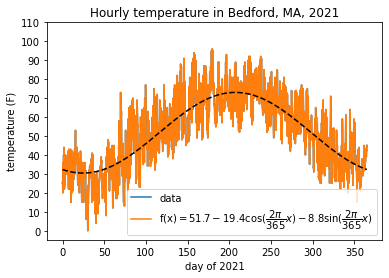
\includegraphics[width=0.45\linewidth]{img/C03weatherBedfordfit.png}
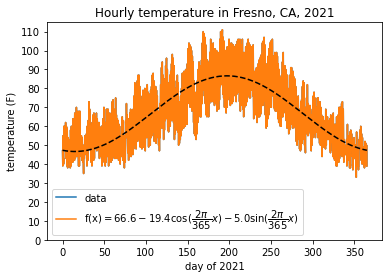
\includegraphics[width=0.45\linewidth]{img/C03weatherFresnofit.png}

\subsection{How is the least squares problem solved?}

\subsubsection{Normal equations}
\noindent\textbf{Choose parameters to minimize the error}
\begin{tcolorbox}
 With $A\vc{w} \approx \vc{y}$, the error is $\vc{e}(\vc{w}) = A\vc{w}-\vc{y}$, and the sum of squared errors is $E(\vc{w}) = \vc{e}(\vc{w})^T\vc{e}(\vc{w})$.
    
    The error function is a scalar function of $\vc{w}$.
    
    By going through an optimization calculation, we'll find that $\vc{w}$ satisfying \[A^TA\vc{w} = A^T\vc{y}\] minimizes the error function.  This system is called the \textbf{normal equations}.  Once we have the normal equations, we can use matrix inversion to set $\vc{w}^* = (A^TA)^{-1}A^T\vc{y}$.
\end{tcolorbox}



To avoid matrix inversion, use a decomposition called a Cholesky decomposition.  This allows us to write $A^TA = LL^T$ where $L$ is lower triangular and $L^T$ is upper triangular.  

What is the advantage of a decomposition into lower and upper triangular matrices?

$LL^T\vc{w}^* = A^T\vc{y}$. Solve this as $L\vc{x} = A^T\vc{y}$ using forward substutition and then $L^T\vc{w}^* = \vc{x}$ using backwards substitution.

\begin{enumerate}[resume=classQ]
\item (Lay 2.5 Q1) Let $A = \left[\begin{array}{r r r}
1 & 0 & 0 \\
-1 & 1 & 0 \\
2 & -1 & 1
\end{array}\right]
\left[\begin{array}{r r r}
1 & -1 & 2 \\
0 & 1 & -1 \\
0 & 0 & 1
\end{array}\right] = LL^T$ and $A^T\vc{y} = \left[\begin{array}{r} 3 \\ -2\\ 6\end{array}\right]$. 

$L$ is a lower triangular matrix and $L^T$ is an upper triangular one.  
\begin{parts}
\item Solve $L\vc{x} = A^T\vc{y}$ for $\vc{x}$.  This is $\left[\begin{array}{r r r}
1 & 0 & 0 \\
-1 & 1 & 0 \\
2 & -1 & 1
\end{array}\right]\vc{x} = \left[\begin{array}{r} 3 \\ -2\\ 6\end{array}\right]$
\item Solve $L^T\vc{w} = \vc{x}$.

\end{parts}
\end{enumerate}

\subsubsection{QR decomposition}

(from Lay \S 6.4)

A matrix $A\in\mathbb{R}^{N\times M}$ with $N>M$ (more rows than columns) and linearly independent columns can be factored as $A = QR$ where the columns of $Q\in\mathbb{R}^{N\times M}$ for an orthonormal basis for $\text{Col} A$ (the span of the columns of $A$), and $R\in \mathbb{R}^{M\times M}$ is an upper triangular invertible matrix with positive entries on the diagonal.

This decomposition is called a $QR$ decomposition.


The orthonormal condition on the columns of $Q$ means $\vc{q}_i\cdot \vc{q}_j = \vc{q}_i^T\vc{q}_j = \delta_{ij}$ and $Q^TQ = I_M$

% $A = \left[\vc{a}_1,\cdots, \vc{a}_M \right]$ and $Q = \left[ \vc{q}_1, \hdots, \vc{q}_M\right]$.

% $\vc{a}_k \in \text{Span}\{\vc{a}_1,...,\vc{a}_M\} = \text{Span}\{\vc{q}_1,...,\vc{q}_M\},$ so we can write \[\vc{a}_k = r_{1k}\vc{q}_1 + ... + r_{kk}\vc{q}_k + 0 \vc{q}_{k+1}+...+0\vc{q}_M\]

% Let $\vc{r}_k = \left[\begin{array}{c}r_{1k} \\ \vdots \\ r_{kk} \\ 0 \\ \vdots \\ 0\end{array}\right]$

% We have $\vc{a}_k = Q\vc{r}_k$ for $k = 1, ..., M$.  Let $R = \left[\vc{r}_1 \cdots \vc{r}_M\right]$.  $A = \left[\vc{a}_1 \cdots \vc{a}_M\right] = \left[Q\vc{r_1} \cdot Q\vc{r}_M\right] = QR$.



% Since $\text{Span}(Q) = \text{Span}(A)$, each column of $A$ can be written as a linear combination of the columns of $Q$.  \[Q^TA = \left[\begin{array}{c c c c}\vc{q}_1^T\vc{a}_1 & \cdots & & \vc{q}_1^T\vc{a}_M \\
% 0 & \vc{q}_2^T\vc{a}_2 & \cdots & \vc{q}_2^T\vc{a}_M \\
% \vdots & \ddots & \ddots & \vdots \\
% 0 & \cdots & 0 & \vc{q}_M^T\vc{a}_M
% \end{array}\right] = QQ^TR = I_m R = R,\] so $R$ encodes the coefficients for those linear combinations.

$Q^TA\vc{w} = Q^T Q R\vc{w} =  R\vc{w} \Rightarrow R\vc{w} = Q^T\vc{y}$.  Because $R$ is upper triangular, $R\vc{w} = Q^T\vc{y}$ can be solved by back-substitution.

\begin{enumerate}[resume=classQ]
\item $\vc{q}_i \in \mathbb{R}^N$ and $\vc{y}\in\mathbb{R}^N$.  
\begin{parts}
\item Is $\vc{y} \in \text{Span}\{\vc{q}_1, ..., \vc{q}_M\}$?  Explain your thinking.
\item Does $\vc{y} = (\vc{y}\cdot\vc{q}_1) \vc{q}_1 + ... + (\vc{y}\cdot\vc{q}_M) \vc{q}_M$?

\item $Q^T\vc{y} = \left[\begin{array}{c} \vc{q}_1^T\vc{y} \\ \vdots \\ \vc{q}_M^T\vc{y}\end{array}\right]$.  What information does this encode?
\end{parts}

\end{enumerate}

\subsubsection{Why have multiple methods?}

Mathematically, any of these systems would allow us to find $\vc{w}^*$.  Once we use computational methods with floating point arithmetic, all of our values are approximate, and the condition number associated with the problem becomes important.

These different methods have different conditioning (error propagation), as well as different numbers of computational steps / computing time.


\subsection{Deriving the normal equations}


 To solve $A\vc{w} = \vc{y}$ in the least squares sense, find $\vc{w}$ that minimizes the error function, $E(\vc{w})$.
    
  Find $\vc{w}$ such that $\dfrac{dE(\vc{w})}{d\vc{w}} = 0$.
  
    \noindent\textbf{Notation}
  \begin{tcolorbox}
      \[\dfrac{dE(\vc{w})}{d\vc{w}}=\left[\begin{array}{ccc} \dfrac{\partial E}{\partial w_1} \hdots \dfrac{\partial E}{\partial w_M} \end{array}\right]\] is also denoted $\left[\text{D}E(\vc{w})\right]$, or simply $\left[\text{D}E\right]$.
      
      Note: $\left[\text{D}E\right]$ is the transpose of $\nabla E$, the gradient of $E$.
  \end{tcolorbox}
  

\noindent\textbf{The normal equations}
\begin{tcolorbox}
Setting $\left[\text{D}E(\vc{w})\right] = \vc{0}$ will result in a matrix equation called the \textbf{normal equations}.  Solving the normal equations for $\vc{w}$ will allow us to find $\vc{w}^*$ or $\hat{\vc{w}}$, the vector that minimizes the error function.
\end{tcolorbox}

\begin{align*}
        E(\vc{w}) &= \vc{e}^T\vc{e} \\
        &=(A\vc{w}-\vc{y})^T(A\vc{w}-\vc{y}) \\
        &=\left((A\vc{w})^T-\vc{y}^T\right)(A\vc{w}-\vc{y}) \\
        &=\left(\vc{w}^TA^T-\vc{y}^T\right)(A\vc{w}-\vc{y}) \\
        &=\left(\vc{w}^TA^T-\vc{y}^T\right)(A\vc{w}-\vc{y}) \\
        &=\vc{w}^TA^TA\vc{w}-\vc{w}^TA^T\vc{y}-\vc{y}^TA\vc{w} + \vc{y}^T\vc{y} \\
        &=\vc{w}^TA^TA\vc{w}-\vc{w}^TA^T\vc{y}-\vc{y}^TA\vc{w} + \vc{y}^T\vc{y}
    \end{align*}
    
\begin{tcolorbox}
    $E(\vc{w})$ is a scalar valued function, so $\vc{w}^TA^T\vc{y}$ is a scalar.  $\vc{w}^TA^T\vc{y}=(\vc{y}^TA\vc{w})^T$.  For any scalar, $\alpha$, we have $\alpha^T = \alpha$.  So $\vc{w}^TA^T\vc{y} = \vc{y}^TA\vc{w}$.  Our error equation becomes
    \[E(\vc{w}) = \vc{w}^TA^TA\vc{w}-2\vc{y}^TA\vc{w} + \vc{y}^T\vc{y}\]
    
To find $\left[\text{D}E\right]$ we will need some facts about matrix derivatives.
\begin{itemize}
\itemsep0pt
    \item $\left[\text{D} A\vc{x}\right] = A$.
    \item (product rule) $\left[\text{D}\left(\vc{u}^T\vc{v}\right)\right]= \vc{u}^T\left[\text{D}\vc{v}\right]+\vc{v}^T\left[\text{D}\vc{u}\right]$
    
    Writing this via dot product notation, for vectors $\vc{u}$ and $\vc{v}$, we have $\left[\text{D}\left(\vc{u}\cdot\vc{v}\right)\right]= \vc{u}\cdot\left[\text{D}\vc{v}\right]+\vc{v}\cdot\left[\text{D}\vc{u}\right]$
\end{itemize}
\end{tcolorbox}

\begin{enumerate}[resume=classQ]
    \item Find the normal equations.  Take all derivatives with respect to $\vc{w}$.
    \begin{parts}
    \item Let $\vc{u} = A\vc{w}$.  Notice that $\left[\text{D} \vc{u}\right] = A$.
    
    
    Rewrite $E(\vc{w})$ in terms of $\vc{u}$.  
    
    \emph{$A$, $A^T$, $\vc{w}^T$, and $\vc{w}$ should all be eliminated so that you have a function of $\vc{u}$ and $\vc{y}$.}

\item Use the product rule and show that $\left[\text{D}E\right] = -2\vc{y}^TA + 2\vc{w}^TA^TA$
    \item Set $\left[\text{D}E\right] = \vc{0}$, take the transpose of both sides, and rearrange to find \[A^TA\vc{w}=A^T\vc{y} \]
   These are the \textbf{normal equations}.
    \item Identify the dimensions of $A^TA$, of $\vc{w}$, and of $A^T\vc{y}$.
    \end{parts}
\end{enumerate}  
  
 
  

    
   
    

% Note: $\varphi_k(x)$ linearly independent means the columns of $A$ are also linearly independent.

% https://math.stackexchange.com/questions/834420/prove-that-ata-is-positive-definite


% \begin{enumerate}[resume=classQ]
% \item Let $E(\vc{w}) = w_1^2+4w_1w_2+3w_2^2+w_2$.  
%  Find $\vc{w}^*$ so that $E(\vc{w}^*)$ is a critical point of the function $E$.
% %\item Recall: $E(\vc{w}^*)$ may be a local minimum, local maximum, or saddle point.  



%\end{parts}


\noindent\textbf{Classifying a critical point}

Let $\vc{w}^*$ be the solution to the normal equations.  Check that $E(\vc{w}^*)$ is a local minimum.
  \vspace{0.2cm}

\begin{tcolorbox}
\begin{itemize}
\itemsep0pt
    \item At a critical point, $\vc{w}^*$, the derivative of the output, $\left[\text{D}E\right]_{\vc{w}^*} = \vc{0}$.  The critical point might be a local minimum, local maximum, or saddle point.
    \item We are looking for a local minimum, so we want $E(\vc{w}^*) < E(\vc{w}^*+\vc{h})$, where $\vc{h}$ is any small vector so $\vc{w}^*+\vc{h}$ is an input close to $\vc{w}^*$.
    
    \item Approximate $E$ at nearby points via Taylor expansion to determine whether $E(\vc{w}^*)$ is a local minimum:
    \[E(\vc{w}^*+\vc{h}) = E(\vc{w}^*) + \left[\text{D}E\right]_{\vc{w}^*}\vc{h} + \frac{1}{2} \vc{h}^T\left[\text{D}^2E\right]_{\vc{w}^*}\vc{h} + \mathcal{O}(\Vert\vc{h}\Vert^3)\]
        \end{itemize}
\end{tcolorbox}


    \begin{tcolorbox}
    \begin{itemize}
  \item  
    At the $\vc{w}^*$ the first derivative, $\left[\text{D}E\right]_{\vc{w}^*}$, is $\vc{0}$, so this simplifies to 
    
    \[E(\vc{w}^*+\vc{h}) = E(\vc{w}^*) +  \frac{1}{2} \vc{h}^T\left[\text{D}^2E\right]_{\vc{w}^*}\vc{h} + \mathcal{O}(\Vert\vc{h}\Vert^3)\]
    \item If $ \vc{h}^T\left[\text{D}^2E\right]_{\vc{w}^*}\vc{h}>0$ for any nonzero perturbation $\vc{h}$ then $E(\vc{w}^*)$ will be a local minimum.
    \end{itemize}
\end{tcolorbox}

\begin{enumerate}[resume=classQ]
    \item (from Lay \S 7.2 Example 6) 
    
    Let $A = \left[\begin{array}{c c c} 3 & 2 & 0 \\ 2 & 2 & 2 \\ 0 & 2 & 1 \end{array} \right]$. Find $\vc{x}^T A \vc{x}$ for each of the following $\vc{x}$. \begin{parts}
    \item Let $\vc{x} = \left[\begin{array}{r} x_1 \\ x_2 \\ x_3 \end{array}\right]$.  
    \item Let $\vc{x} = \left[\begin{array}{r} 1 \\ -2 \\ 2\end{array}\right]$. 
    
    \item Let $\vc{x} = \left[\begin{array}{r} 2 \\ -1 \\ -2\end{array}\right]$.  
    \end{parts} 
    
    
\end{enumerate}
\begin{tcolorbox}
\begin{itemize}
\itemsep0pt
    \item A weighted sum of quadratic terms, $Q(\vc{x}) = \sum\limits_{j=1}^n\sum\limits_{k=1}^n q_{jk}x_jx_k$, can be encoded as an expression of the form $\vc{x}^TA\vc{x}$ where $A$ is an $n\times n $ symmetric matrix.
    \item The function $Q(\vc{x})$ is called a \textbf{quadratic form}.
    \item 
The matrix $A$ is called the \textbf{matrix of the quadratic form}.
\end{itemize}
\end{tcolorbox}

\begin{enumerate}[resume=classQ]
    \item (Lay \S 7.2 Q3a) 
    Find the matrix of the quadratic form $10x_1^2 - 6x_1x_2 - 3x_2^2$ (assume $\vc{x}\in\mathbb{R}^2$).
\end{enumerate}



\begin{tcolorbox}
    \begin{itemize}
    \item If a change of variables $\vc{x} = P\vc{y}$ is made in the quadratic form $\vc{x}^TA\vc{x}$ then
    \[\vc{x}^TA\vc{x} = (P\vc{y})^TA(P\vc{y}) = \vc{y}^TP^TAP\vc{y} = \vc{y}^T(P^TAP)\vc{y}\]
    \item $A$ is a symmetric matrix, so it is orthogonally diagonalizable.  It can be written in the form $A = PDP^T$ where $P$ is an orthogonal matrix (so $P^T=P^{-1}$), and $D$ is a diagonal matrix.  With $\vc{x} = P\vc{y}$, we have $\vc{x}^T A \vc{x} = \vc{y}^T D \vc{y} = \sum\limits_{i=1}^n \lambda_i y_i^2$.
    
    \item A symmetric matrix $A$ where $\vc{h}^TA\vc{h}>0$ for all nonzero $\vc{h}$ is called \textbf{positive definite}.
    
    A symmetric matrix $A$ is positive definite if and only if the eigenvalues of $A$ are positive.
 
    
    \item $\left[\text{D}^2E\right]_{\vc{w}^*} = \left[\begin{array}{ccc}
    \dfrac{\partial^2E}{\partial w_1 \partial w_1} & \hdots & \dfrac{\partial^2E}{\partial w_1 \partial w_M} \\
    \vdots & \ddots & \vdots \\
    
    \dfrac{\partial^2E}{\partial w_M \partial w_1} & \hdots & \dfrac{\partial^2E}{\partial w_M \partial w_M}
    \end{array}\right]$. This is the \textbf{Hessian} matrix.  The equality of mixed partials means that the Hessian matrix is symmetric.
    \item $\vc{w}^*$ will be a local minimum if the Hessian matrix, evaluated at $\vc{w}^*$, is positive definite (i.e. has positive eigenvalues).
\end{itemize}
\end{tcolorbox}
\begin{enumerate}[resume=classQ]
\item Let $E(\vc{w}) = w_1^2+4w_1w_2+3w_2^2+w_2$.  
 
% You found a critical point $(w_1, w_2)^*$ above.  
 \begin{parts}
 \item Find a critical point.
\item  Find the Hessian matrix, evaluated at this critical point.
\item The determinant of a matrix gives the product of the eigenvalues, $\lambda_1\lambda_2$.  The trace of a matrix gives the sum of the eigenvalues, $\lambda_1+\lambda_2$.  For a $2\times 2$ matrix this information is sufficient to determine the sign of the eigenvalues.  

Find the determinant of the Hessian (and the trace if necessary) to determine the sign(s) of the eigenvalues.  Use this to classify the critical point.
 \end{parts}
 




%\end{parts}

\end{enumerate}


\section{Condition number in matrix problems}

So far we have assumed all the math is being done exactly (without the approximations intrinsic to floating point representations and calculations).

\vspace{0.2cm}

\noindent\textbf{Conditioning}
\begin{tcolorbox}
\begin{itemize}
\itemsep0pt
\item Let $A\vc{x} = \vc{b}$ where $A$ is $n\times n$ and invertible.  $A(\vc{x} + \delta\vc{x}) = \vc{b} + A\delta\vc{x}$ (by linearity) so $\delta\vc{b} = A\delta\vc{x}$.
    \item The condition number is $\dfrac{\Vert \delta \vc{b}\Vert/\Vert\vc{b}\Vert}{\Vert \delta \vc{x}\Vert/\Vert\vc{x}\Vert} = \dfrac{\Vert \delta \vc{b}\Vert}{\Vert\delta\vc{x}\Vert}\dfrac{\Vert \vc{x}\Vert}{\Vert\vc{b}\Vert} = \dfrac{\Vert A\delta \vc{x}\Vert}{\Vert\delta\vc{x}\Vert}\dfrac{\Vert A^{-1}\vc{b}\Vert}{\Vert\vc{b}\Vert}$.  For a matrix we define $\Vert A\Vert = \max\limits_{\vc{x}}\dfrac{\Vert A\vc{x}\Vert}{\Vert\vc{x}\Vert}$.
   \end{itemize} 
 \end{tcolorbox}   
 \begin{tcolorbox}
   \begin{itemize}
\itemsep0pt
   \item  $\dfrac{\Vert \delta \vc{b}\Vert/\Vert\vc{b}\Vert}{\Vert \delta \vc{x}\Vert/\Vert\vc{x}\Vert} = \dfrac{\Vert A\delta \vc{x}\Vert}{\Vert\delta\vc{x}\Vert}\dfrac{\Vert A^{-1}\vc{b}\Vert}{\Vert\vc{b}\Vert}\leq \Vert A\Vert \Vert A^{-1}\Vert$.
   \item  Define the \textbf{condition number} of a matrix as $\kappa(A) =\Vert A\Vert\Vert A^{-1}\Vert$
   \item The condition number of a matrix satisfies.  $1\leq \kappa(A) < \infty$, and we'll call a problem \textbf{well conditioned} if $\kappa(A)$ is not too large.
   \item  Notice that the condition number bounds  $\dfrac{\Vert \delta \vc{b}\Vert/\Vert\vc{b}\Vert}{\Vert \delta \vc{x}\Vert/\Vert\vc{x}\Vert}$ and $\dfrac{\Vert \delta \vc{x}\Vert/\Vert\vc{x}\Vert}{\Vert \delta \vc{b}\Vert/\Vert\vc{b}\Vert}$ identically.  $ \dfrac{\Vert \delta \vc{x}\Vert/\Vert\vc{x}\Vert}{\Vert \delta \vc{b}\Vert/\Vert\vc{b}\Vert}= \dfrac{\Vert A^{-1}\delta \vc{b}\Vert}{\Vert \delta\vc{b}\Vert}\dfrac{\Vert \vc{Ax}\Vert}{\Vert\vc{x}\Vert}\leq \Vert A\Vert \Vert A^{-1}\Vert$
   \item For an $N\times M$ matrix, we will need a slightly different definition (it will be analogous, but will avoid $\Vert A^{-1}\Vert$, since that is undefined in the non-square matrix case.
\end{itemize}
 \end{tcolorbox}



%\section{QR}. 

\end{document}
